\chapter{Introduction}\label{ch:1}

%section 1.1 begins %%%%%%%%%%%%%%%%%%%%%%%%%%%%%%%%%%%%%%%%%%%%%%%%%%%%%%%%%%%%%%%%%%%%
\section{An interest sparked} \label{1.1}
The summer of 2004 marked the first time I, as a then undergraduate student, had ever set foot on Surinamese soil. The purpose of the trip was to collect language data on the English-lexicon creoles spoken in the country. In analysing the data collected, I began to unearth various correspondences between the phonetic shapes of words of English origin and their reflexes across Saramaccan, Sranan, and Aukan, hereafter \textsc{ssa}.

In March of 2007, I, as a graduate student supervising an undergraduate fieldtrip, went to Suriname again. On that occasion, I was fortunate enough to be able to collect additional data from other \textsc{ssa}  settlements not previously visited during the 2004 fieldtrip. On this occasion, the goal was to determine to what degree the phenomena noticed on the 2004 fieldtrip were similar across different groups of \textsc{ssa}  speakers. I noticed the same phonetic correspondences as well as new ones across the various \textsc{ssa}  reflexes and their English cognates.

One correspondence observed was the production and non-production of /r/ in post-vocalic positions. Some \textsc{ssa}  words such as Sranan's \emph{more} [\textipa{moro}], Saramaccan's \emph{work} [\textipa{woroko}] and Aukan's  \emph{gutter} [\textipa{gotro}] suggested that the English input forms had a postvocalic /r/, hereafter \textsc{pvr}. However, other words such as Sranan's \emph{four} [\textipa{fO}], Saramaccan's \emph{finger} [\textipa{fINga}] and Aukan's \emph{horse} [\textipa{asI}] suggested that other English input forms lacked a post-vocalic /r/; I was fascinated and my fascination led me to ask three questions:

\begin{enumerate}
\item Was \textsc{ssa}  influenced by both /r/-full and /r/-less British Isles English dialects?
\item Was \textsc{ssa}  influenced by both /r/-full and /r/-less British Isles English dialects?
\item Was the combination /r/-fullness and /r/-lessness a purely Sranan phenomenon?
\end{enumerate}

I had a desire to know more; I needed to know the exact origin of the patterns of correspondence and lack of correspondence thereof, with rhotic dialects of English and \textsc{ssa}. I also needed to ascertain why these and other patterns presented themselves across all three creoles. This linguistic curiosity led to my perusing both historical and historical-linguistic works about \textsc{ssa}  and Suriname; some of these included: \citet{Bridenbaugh68},  \citet{Esposito82},   \citet{Hoefte98}, \citet{Kambel99},  \citet{Rens53},  \citet{Muysken86},  \citet{Smith87} and   \citet{Smith01}.

The insights gained from these works did their part in fuelling my interest even further. I had been working on another research topic for my dissertation, but I dropped it. I wanted to pursue my \textsc{ssa}  interest, specifically my interest in Suriname's lingua franca, Sranan, which was the main \textsc{ssa}  creole that I was researching during the two above-mentioned fieldtrips. With my change in interest from my previous topic and after spending years scrutinizing Sranan data, English dialectal geography data in the form of The Survey of English Dialects  \citep{Orton6271}, and 17\textsuperscript{th} century historical data from England, I broadened the focus of the research and this led to the following research questions:

\begin{enumerate}
\item What do lexico-phonetic correspondences between Sranan words and their English dialectal etyma tell us about where within England this influence might have originated?
\item What can one (1.) above tell us about the competing hypotheses concerning the source of lexico-phonetic input in Sranan, i.e. a pan-dialectal account versus a mono-dialectal account?
\item What kind of corroboration for or challenge to the proposed dialect area(s) do we find in the historical records?
\end{enumerate}

The data and method used to address these research questions are outlined in more detail in \chapref{ch:3}. The remainder of this chapter is a presentation of a brief history of Suriname and the \textsc{ssa}  creoles, specifically Sranan; the major problem that the research addresses, the significance of the research and an outline of the contents of the remaining chapters.
%section 1.1 ends %%%%%%%%%%%%%%%%%%%%%%%%%%%%%%%%%%%%%%%%%%%%%%%%%%%%%%%%%%%%%%%%%%%%%

%section 1.2 begins %%%%%%%%%%%%%%%%%%%%%%%%%%%%%%%%%%%%%%%%%%%%%%%%%%%%%%%%%%%%%%%%%%%%

\section{Brief history of Suriname and Sranan} \label{1.2}
\subsection{The seventeenth century settlers} \label{1.2.1}

The English arrived in the West Indies in 1624, settling first in St. Christopher, present day St. Kitts. They subsequently settled Barbados in 1627  \citep[18]{Dunn73}, Nevis in 1628  \citep[297]{Wroughton06}, and Antigua and Montserrat in 1632, respectively \citep[27]{Forsyth69}. Of these settlements Barbados, by the 1650s, had the largest population. Its importance among the English colonies grew steadily and Barbados soon took over the function of a way station from St. Kitts, but on a far greater scale \citep{Davies74}. Between 1650 and 1680, for example, Barbados, with its ``... swiftly acquired white population, [which was] made increasingly redundant ... after 1640 by the introduction of slave labor ... may have supplied to buccaneering, to expeditionary forces out of England, and to colonies as many as 20,000 ... [or possibly] ... 30,000 ..." people \citep[137]{Davies74}. Suriname was one of the colonies settled from Barbados.

British colonists, sanctioned by Lord Francis Willoughby, governor of Barbados, settled Suriname from Barbados in the early 1650s \citep{Ehrlich09, Arbell02, Hyamson08}, after two failed attempts to do so in 1630 and 1649 \citep[82]{Arbell02}. Three hundred Barbadians under the command of soon to be governor, Anthony Rowse, ``landed on the Surinam and Commewine rivers?" and, after making peace with the native Amerindians, gave the English a stable footing in the mainland territory \citep[414]{Salomon99}. Suriname would soon become a thriving colony due to continual migration from Barbados. By 1663, for example, the Suriname colony ``... boasted a population of 1,000 Whites, 2,000 enslaved Africans and 1,000 natives scattered among fifty large and several smaller plantations" \citep[808]{Marley05}.

In 1664, when the French captured nearby Cayenne from the Dutch, the Portuguese Jews and their enslaved Africans who resided there were forced to move into Suriname \citep{Redfield00, Friedman99}. Willoughby granted them permission to settle in Suriname since their affluence and planting expertise rendered them an asset to the colony \citep{Ehrlich09}. Consequently, by 1667, of the one hundred and eighty plantations in Suriname, six or seven of them belonged to these Portuguese Jews \citep{Arbell02, Rens53}. These Jewish plantations, though separate from the English plantations, were located in a cluster in close proximity to the English ones. All one hundred and eighty plantations were located along the coastal area between the Cassipora creek, nowadays known as Joden Savanne, and Torarica, approximately 40 km south of Paramaribo (see \figref{Map1.1} on page \pageref{Map1.1}).

\begin{figure}
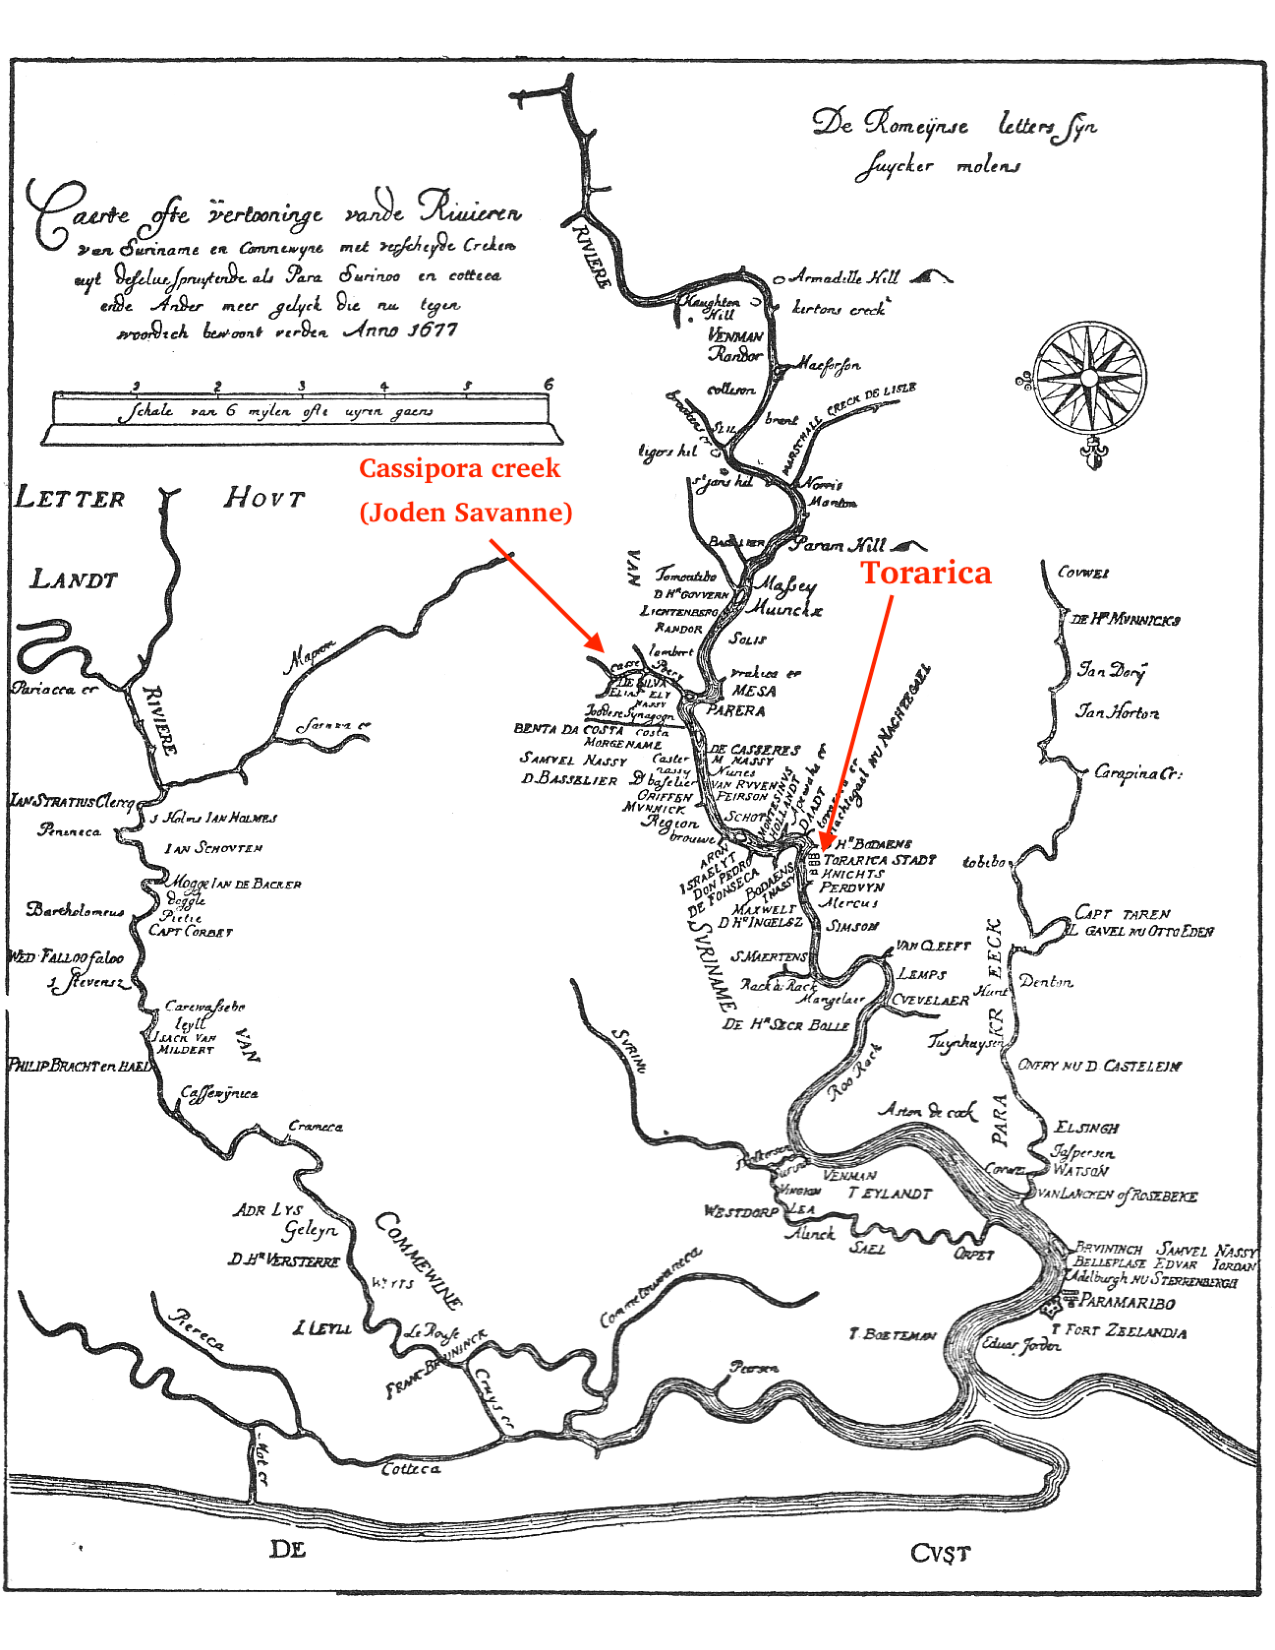
\includegraphics[width=\textwidth] {figures/1677kaartSurinameMogge.pdf}
% % % \captionsetup{name=Map}%
\caption {Location of plantations in late 17\textsuperscript{th} century Suriname. Source: \citet{Mogge77}} 
\label{Map1.1}
\end{figure}


In 1667, the Dutch, led by Abraham Crijnssen, conquered Suriname during the second Anglo-Dutch War of 1665 to 1667. According to \citet{Hoefte98}, this war began because England attempted to terminate the Dutch dominance over world trade routes. On July 31, 1667, via the peace treaty of Breda, Suriname was ceded to the Dutch in exchange for New Amsterdam, which is present day New York \citep{Kaufman05}. Consequently, as allowed under the conventions of the Treaty of Breda \citep[617--618]{gbhol61}, most of the English planters with enslaved Africans purchased before the cession to the Dutch, alongside indentured servants and free Whites, began leaving the mainland colony between 1668 and 1675 \citep{Arbell02, Faber98, Godfrey95}.

What was the linguistic situation while the English were in control of the colony? How did this linguistic situation change with the arrival and subsequent settlement of the Portuguese? What happened after the departure of the English and arrival of the Dutch and how did these social and linguistic changes contribute to the development of Sranan Tongo?

\subsection {A change in the linguistic ecology of Suriname}\label{1.2.2}
The English population in Suriname, up until the commencement of their departure after 1667, consisted of planters, free Whites and indentured servants who were coming from Barbados \citep{Arbell02, Sainsbury80}. During the period of English control, specifically between the period 1650 to 1664, i.e. the period prior to the introduction of the Portuguese element into the colony, indentured servants from within the British Isles constituted the bulk of the population in the English colonies \citep{Kenny06, Powell05, Armitage05}. This is linguistically significant because these indentured servants ``formed the primary [English Superstrate] linguistic models'' \citep[117]{Arends02} for the enslaved Africans with whom they worked side by side on the plantations \citep{Galenson02}.

According to \citet{Rens53}, among the settlers going to Suriname from Barbados, some might have previously been residents of St. Kitts. This, according to \citet[117]{Arends02}, is very significant because St. Kitts was not only the first colony to be colonised by the English, but it ``... may [also] have been the centre of diffusion of restructured English throughout the Caribbean, including Barbados.'' It seems that it is for this reason that \citet{Arends02} holds the view that the English roots of the Surinamese English-lexicon creoles should not be sought in Barbados but in St. Kitts. I agree with \citet{Arends02} to an extent. However, given the migration patterns of indentured labourers from England during the period in which Suriname was settled, I would argue that \textsc{ssa}'s English linguistic influence is a combination of St. Kitts'  ``restructured English'', alongside the linguistic influence(s) from the indentured servants who arrived in Barbados during the early 1650s onwards (see \chapref{ch:6}).

The linguistic ecology of Suriname changed after 1664 with the arrival of the Portuguese Jews, who established their plantations in close proximity to the English ones. The subsequent linguistic situation had an effect on the \textsc{ssa}  creole languages albeit in varying degrees (see \tabref{Table1.1}). According to \citet{Rens53}, the ``\ili{Neger-English}''  that was spoken in the colony by both the English and enslaved Africans went through a process of fusion with the Portuguese linguistic systems that the Portuguese Jews and the enslaved took with them to Suriname.

The linguistic ecology in Suriname changed again in 1667 with the cession of the colony by the English to the Dutch. Barring runaway slaves, some of whom spoke ``\ili{Neger-English}'' and the few English who had stayed, with most of the English indentured servants, planters and ``\ili{Neger-English}''-speaking enslaved Africans leaving the colony, Suriname's linguistic ecology soon changed to one dominated by Portuguese and Dutch. Intriguingly, ``as far as the lexicons of the Surinamese Creoles are concerned, it is an undisputed fact that English ... [had] ... played a major role in their composition'' \citep[117]{Arends02}. Irrespective of the Portuguese and Dutch linguistic influences from 1667 onwards, the English element was so deeply entrenched in the \textsc{ssa} creole languages that even to date they can still be classified as English-lexicon creole languages; this is illustrated in \tabref{Table1.1} below.

\begin{table}
\begin{tabular}{lrrrr} 
\lsptoprule
\textbf& English  & Portuguese  & Dutch &  West African  \\
\midrule
Sranan &  71.40\% & 3.70\% & 17.85\% & 1.59\%  \\
Aukan &  76.47\% & 5.04\% & 15.97\% & 2.52\%  \\
Saramaccan & 49.96\% & 34.88\% & 10.45\% & 4.74\%  \\  
\lspbottomrule 
\end{tabular}
\caption{Lexical sources of the 200-word basic vocabulary list for \textsc{ssa} }
\label{Table1.1}
\end{table}

 \tabref{Table1.1} does more than highlight the significance of the English element based on a look at the 200-word basic vocabulary for the \textsc{ssa}  creole languages; the table also highlights the fact that Dutch had little linguistic influence on the \textsc{ssa}  creole languages. This lack of significant linguistic influence from Dutch is possibly attributable to the fact that the Dutch were never able to implement, with any degree of success, the system of indentured servitude that the British were able to establish \citep{Buddingh95}. Added to this is the fact that even though Dutch became the official language of the colony and the ``language of literacy after emancipation,'' it was a language of high status that was seldom used to communicate with speakers of Sranan (whether enslaved Africans or any of the English who were in the country) during the 17\textsuperscript{th} and 18\textsuperscript{th} century \citep[279]{Healy93}.

The table also highlights another interesting fact, i.e. that the Portuguese element, based on the 200-word basic vocabulary list, is far greater in Saramaccan than the other two \textsc{ssa}  creoles. This has led some linguists, such as  \citet{Perl95}, to suggest that Saramaccan should be classified as a Portuguese-lexicon creole language. Though this is not a position that I hold, this current work is not the medium through which to contest this claim. Let us therefore move to a brief discussion of the linguistic development of \textsc{ssa}.

\subsection {Linguistic development of \textsc{ssa} }\label{1.2.3}
There are a number of elaborate explanations that various linguists have provided concerning the development of the \textsc{ssa}  creole languages. This dissertation does not concern itself with which of these explanations is more valid and/or trustworthy. For this reason, the discussion hereafter is but a brief presentation of a few of them.

There are two major hypotheses that attempt to account for the development of the \textsc{ssa}  creole languages; these are the Parallel Origin Hypothesis and the Serial Origin hypothesis \citep{Smith01}. According to the Parallel Origin Hypothesis, Proto-Sranan, Proto-Saramaccan and Proto-Aukan developed independently, albeit from some type of Caribbean Plantation Pidgin English, hereafter \textsc{cppe}, which might have existed in the English colonies during the first generation of slavery  \citep{Smith01, McWhorter98}. \textsc{cppe} possibly originated from an English pidgin that might have been developed and spoken by castle slaves along the West African slave settlements \citep{McWhorter00b}.

According to \citet{McWhorter00b}, since all Atlantic English Creoles ``... must trace to a single ancestor, it is most likely that the pidgin was transported to ... St. Kitts and Barbados [which were]... the first colonies settled [by the English] and the source of settlers and slaves to subsequent [English] colonies ...'' (111). This transported English pidgin was possibly the same ``... embryonic Medium for Inter-ethnic Communication ...'' which according to \citet[347]{Baker98} existed in 1620s St. Kitts long before it became a first language and was spread to the other English territories. In all likelihood \textsc{cppe} is the same as Baker's proposed mixed Afro-English communication system \citep{Baker98}, which was spread to the other British colonies including Suriname; \textsc{cppe} might also be a further developed version of Baker’s Medium for Inter-ethnic Communication \citep{Baker98}, which developed due to the influence of the indentured servants coming into the colonies from the 1650s onwards (see \chapref{ch:6}).

The Serial Origin hypothesis also attributes the development of \textsc{ssa}  to \textsc{cppe}. However, Proto-Sranan is considered to be the first to develop from \textsc{cppe}, within Suriname, followed by Aukan and Saramaccan as offshoots from Sranan \citep{Smith01, McWhorter98}. Shortly after \textsc{cppe} was transported to Suriname, Sranan developed, before Saramaccan and Aukan, due to the continual contact between enslaved Africans, ``... indentured servants and poor whites, who acted as bookkeepers and overseers on the plantations ...'' \citep[xii]{Cassidy67}. This English, indentured servant-based, linguistic influence would certainly have lasted only until just after 1668, with the departure of the English.

\citet{Smith09, Smith06, Smith02} argued that Sranan developed in the first half of the 1660s. In fact, \citet[316]{Smith09} ``... [dated] the creolization of Sranan at 1660--1665.'' This means that by the time of the arrival of the Portuguese Jews in 1664, Sranan or some semblance of it was already created. Smith's claim is supported by \citet[28]{Rens53} who claimed that prior to the arrival of the Portuguese Jews in Suriname, ``\ili{Neger-English}'' had long been established among the enslaved Africans and white inhabitants of the country.

Sranan, by around 1680--1690, was partly relexified by Portuguese. This is attributed to the influence of Portuguese Jewish immigrants who were granted asylum in 1664  \citep{McWhorter11, Smith06, Holm89}. According to  \citet[156]{Smith08b}, these Portuguese Jews had brought ``Portuguese speaking slaves with them to Suriname'' when they first entered the then English colony. At some point there was a fusion of what \citet{Rens53} called Neger-Portuguese, spoken by the Portuguese enslaved Africans, and the \ili{Neger-English} spoken by the English enslaved Africans and some of the indentured servants. This possibly took place during and after 1667, when the Portuguese Jews purchased Sranan (\ili{Neger-English}) speaking enslaved Africans from the English who were preparing to migrate from Suriname due to its having been ceded to the Dutch \citep{Ehrlich09, Mufwene01, Friedman99, McWhorter98, Wurm96, Rens53}. This fusion of the two languages saw the birth of a kind of Dju-Tongo (Jew language), a mixed Portuguese/English creole, in the middle of the Suriname River plantations \citep{Arends95}.

By the 1690s, the first group of enslaved Africans ran away from the Portuguese Jewish plantations to form the first Saramaccan group in the interior of the country \citep{Huber99}. The high percentage of Portuguese lexical items in Saramaccan (see \tabref{Table1.1} on Page~\pageref{Table1.1}) is attributed to this Dju-Tongo, which according to \citet{Arends95} ``... [involved] the same mix of English, Portuguese and African elements as Saramaccan...'' (169).

Aukan (commonly referred to as Ndjuka or Djuka) ``... is lexically more similar to Sranan''  \citep[Introduction]{Huttar94}. \citet{Huttar94} claimed that this creole language variety appeared in the first half of the 18\textsuperscript{th} century, when ``large numbers of slaves escaped from plantations chiefly along the Cottica and Commewijne rivers where a contact language drawing much of its lexicon from English was in use'' \citep[Introduction]{Huttar94}. This contact language is what \citet{McWhorter98}  considered to be Sranan.

Since most of the English would have already migrated from Suriname by 1680, resulting in Sranan's linguistic ecology being one that was dominated by Portuguese and Dutch, how do we account for Aukan being similar to Sranan? How can we account for Sranan still being spoken as the lingua franca today, as opposed to Saramaccan or some Dutch-based creole that is a fusion of Dutch and \ili{Neger-English} (Sranan)? According to \citet{Holm94} the Dutch in Suriname treated Sranan as a language in its own right, though not one of prestige. Consequently, they learned it as a second language to communicate with their enslaved Africans, some of whom were acquired from the migrating English after Suriname?s cession to the Dutch (see \chapref{ch:6}).

This work does not attempt to settle which of the two hypotheses, i.e. the Parallel Origin Hypothesis or the Serial Origin Hypothesis, is more trustworthy. What is important is the fact that \textsc{ssa}, specifically Sranan, contains what might be considered ``fossilized'' linguistic remnants of an early English colonial period. Therefore, it is being proposed here, that these linguistic ``fossils'' can be used to trace the dialect origin(s), in England, of the early English influence.
%section 1.2 ends %%%%%%%%%%%%%%%%%%%%%%%%%%%%%%%%%%%%%%%%%%%%%%%%%%%%%%%%%%%%%%%%%%%%%

%section 1.3 starts %%%%%%%%%%%%%%%%%%%%%%%%%%%%%%%%%%%%%%%%%%%%%%%%%%%%%%%%%%%%%%%%%%%%%
\section{The problem} \label{1.3}

Though linguists, such as \citet{Smith08, Smith87} and \citet{Mufwene08, Mufwene01}, present 17\textsuperscript{th} century dialects of English as the lexical input for English creoles, Smith was more specific regarding the nature of this input. He posited dialect levelling involving an approximation of an emerging 17\textsuperscript{th} century ``... London English, primarily Standard Early Modern English ...'' \citep[118]{Smith08}. He held this view because he believed that ``... the English that developed in the general London area [was] ancestral to all forms of English developed external to the British Isles ...'' \citep[118]{Smith08}. He supported this claim by tracing systematic sound changes based on south-east England English input and their realisations in Suriname. \citet{Smith08, Smith87} did not, however, present evidence to repudiate the possibility of a pan-dialectal account of origin, i.e. the possibility that the origin of this influence was coming from dialects from all over England. This latter view is endorsed by \citet{Mufwene08, Mufwene01}.

\citet{Mufwene08, Mufwene01} believed that ``... the target for those who made the creoles, consisted of several non-standard [dialect] varieties [of the European lexifiers that were] competing with each other ...'' \citep[21]{Mufwene08}. Like \citet{Smith08, Smith87}, \citet{Mufwene08, Mufwene01} failed to provide any assessment of the possibility of an alternative account to his pan-dialectal one; i.e. he did not address the possibility of a mono-dialectal source of origin, such as that proposed by \citet{Smith08, Smith87}.
%section 1.3 ends %%%%%%%%%%%%%%%%%%%%%%%%%%%%%%%%%%%%%%%%%%%%%%%%%%%%%%%%%%%%%%%%%%%%%

%section 1.4 starts %%%%%%%%%%%%%%%%%%%%%%%%%%%%%%%%%%%%%%%%%%%%%%%%%%%%%%%%%%%%%%%%%%%%%
\section {Significance of research}\label{1.4}
This research attempts to settle the pan-dialectal and the mono-dialectal contention surrounding the nature of the historical lexico-phonetic input in English creoles, specifically Sranan. To this end, it puts forward a methodological apparatus that one can use to undertake such reconstructive work and achieve replicable results. This methodological tool involves a combination of statistics (\chapref{ch:4}), English dialect geography (\chapref{ch:5}) and 17\textsuperscript{th} century history of England (\chapref{ch:6}).
%section 1.4 ends %%%%%%%%%%%%%%%%%%%%%%%%%%%%%%%%%%%%%%%%%%%%%%%%%%%%%%%%%%%%%%%%%%%%%

%section 1.5 starts %%%%%%%%%%%%%%%%%%%%%%%%%%%%%%%%%%%%%%%%%%%%%%%%%%%%%%%%%%%%%%%%%%%%%
\section{Outline of chapters}\label{1.5}
\chapref{ch:2}, \emph{Brief overview: Views on superstrate influence}, begins with a brief discussion of the theories of creole genesis that exist to date. The discussion then looks specifically at two superstratist approaches of origin which offer opposing ideas about the nature of the superstrate input; it then focuses specifically on the superstrate influence in Sranan. The discussion concludes with an explanation and rationale for the direction that this research takes in attempting to establish what Sranan's linguistic influence from England looks like and how best to account for it.

\chapref{ch:3}, \emph{About the data and research design}, is divided into two major sections. The first section, \emph{Data Sources}, is a discussion and presentation of the Sranan, the English of England, 17\textsuperscript{th} century history of England data sources and the linguistic features assessed in this research. The second section, \emph{Research Design}, is a detailed discussion and presentation of:

\begin{enumerate}
\renewcommand{\labelenumi}{\alph{enumi}.} 
\item the approach taken in gathering, organising and using the English regional dialect data and the Sranan data; and
\item the processes that took place at each stage of the proposed tripartite methodological model used to undertake this research.
\end{enumerate}

\chapref{ch:4}, \emph{Testing probability of origin}, is a presentation of the statistical component of the methodological apparatus at work, using 45 putative lexico-phonetic English etyma, hereafter the \textsc{\emph{sed45}}, which have been selected for this research (see \chapref{ch:3}). The chapter discusses the probability of finding a single dialect locality of origin, which exhibits a high degree of correspondence between the 45 putative input etyma and their Sranan reflexes, hereafter referred to as the Sranan45. It then looks at the significance of actually finding a single such locality of origin from within England and subsequently presents the actual results of the statistical analysis.

\chapref{ch:5}, \emph{A dialect geography approach}, is a presentation and discussion of potential locations of origin in England of the English reflexes for the Sranan45. In this chapter, the results of the statistical analysis presented in \chapref{ch:4} are temporarily disregarded and the data are analysed anew within a dialect geography framework. This involves plotting on a map of England the geo-linguistic distribution of the \textsc{\emph{sed45}} etyma. The chapter concludes with a discussion of the degree of corroboration between the results of the geo-linguistic mapping and the results of the statistical analysis of the  \textsc{\emph{sed45}}.

\chapref{ch:6}, \emph{The historical complement}, is a discussion of the 17\textsuperscript{th} century migration patterns of people from England going to British colonies in the Americas. The focus of the discussion is on the patterns of migration from the locations identified via the statistical analysis and the geo-linguistic mapping as the potential sources for the Sranan45. The discussion is concerned with answering three main questions that are posed at the end of \chapref{ch:5}. These are as follows:

\begin{enumerate}
\item Can we establish a chain of migration from England to Suriname, between the periods 1650--1667?
\item Can we establish a chain of migration from England, within the same time span mentioned in (1), to the English colonies in the Caribbean and subsequently Suriname?
\item Can we, if the answer(s) to (1) and/or (2) is/are in the affirmative, then determine what percentage of the total number of migrants to the Caribbean, including Suriname, is from the localities pinpointed in Chapters~\ref{ch:4} and~\ref{ch:5}?
\end{enumerate}

\chapref{ch:7}, \emph{A Tale of Two Dialect Inputs}, is a discussion of the composite findings from the three components of the analytical tool (see Chapters~\ref{ch:4}--\ref{ch:6}). This final chapter also looks at the significance of these combined findings as they relate to Sranan, Linguistic reconstruction, Dialect geography, Creole and Historical Linguistics and English-lexicon creole languages in general.
%section 1.5 ends %%%%%%%%%%%%%%%%%%%%%%%%%%%%%%%%%%%%%%%%%%%%%%%%%%%%%%%%%%%%%%%%%%%%%
